% Copyright 2026 Fausto Spoto
%
% Licensed under the Apache License, Version 2.0 (the "License");
% you may not use this file except in compliance with the License.
% You may obtain a copy of the License at
%
%    http://www.apache.org/licenses/LICENSE-2.0
%
% Unless required by applicable law or agreed to in writing, software
% distributed under the License is distributed on an "AS IS" BASIS,
% WITHOUT WARRANTIES OR CONDITIONS OF ANY KIND, either express or implied.
% See the License for the specific language governing permissions and
% limitations under the License.

%\RequirePackage{luatex85}
\documentclass[11pt]{beamer}  %% versione proiettore
%%\documentclass[11pt,handout]{beamer} %% versione stampa
\usepackage{lucidiJb-2ed}

\usepackage{animate}
\usepackage{mathtools}
\usepackage{relsize}
\usepackage[normalem]{ulem}
\usepackage[dvipsnames]{xcolor}
\usepackage{amsmath}
\usepackage{amssymb}
\usepackage{amsfonts}
\usepackage{tikz}
%\usetikzlibrary {arrows.meta,graphs,graphdrawing}
%\usegdlibrary{layered}
%\usegdlibrary{trees}
\usetikzlibrary{decorations.pathreplacing}
\usetikzlibrary {arrows.meta}
\usepackage{algorithm,algpseudocode}
\usepackage{listings}

\lstset{
  breakatwhitespace,
  language=MATLAB,
  columns=fullflexible,
  keepspaces,
  breaklines,
  tabsize=3, 
  showstringspaces=false,
  extendedchars=true,
  basicstyle=\fontfamily{pcr}\selectfont\scriptsize,
  keywordstyle=\color{orange},
  upquote=true,
  literate={-}{-}1}

\renewcommand{\algorithmicrequire}{\textbf{Input:}}
\renewcommand{\algorithmicensure}{\textbf{Output:}}

\mode<article>
{
  \usepackage{fullpage}
  \usepackage{hyperref}
}

\mode<presentation>
{
  \setbeamertemplate{background canvas}[vertical shading][bottom=red!10,top=blue!10]
  \usetheme{Course}
  \usefonttheme[onlysmall]{structurebold}
}

\colorlet{verylightviolet}{violet!20!white}
\colorlet{verylightred}{red!20!white}

\newcommand{\db}{
\includegraphics[width=1.3cm]{pictures/db}}
\newcommand{\computer}{
\includegraphics[width=1.3cm]{pictures/computer}}
\newcommand{\phone}{
\includegraphics[width=1.3cm]{pictures/phone}}

\newcommand{\wrt}{\textit{wrt.\ }}
\newcommand{\ie}{, \textit{ie.}, }

\newcommand{\numberofscoops}{{\#\mathit{scoops}}}
\newcommand{\noncesize}{{\mathit{nonce}_{\mathit{size}}}}
\newcommand{\byte}{{\mathit{byte}}}
\newcommand{\nonce}{{\mathit{nonce}}}
\newcommand{\bestNonce}{{\mathit{best\_nonce}}}
\newcommand{\nonces}{{\mathit{nonces}}}
\newcommand{\scoops}{{\mathit{scoops}}}
\newcommand{\plot}{{\mathit{plot}}}
\newcommand{\scoop}{{\mathit{scoop}}}
\newcommand{\seed}{{\mathit{seed}}}
\newcommand{\previous}{{\mathit{previous}}}
\newcommand{\deadline}{{\mathit{deadline}}}
\newcommand{\generation}{{\mathit{generation}}}
\newcommand{\size}{{\mathit{size}}}
\newcommand{\scoopnumber}{{\mathit{scoopNumber}}}
\newcommand{\data}{{\mathit{data}}}
\newcommand{\challenge}{{\mathit{challenge}}}
\newcommand{\delay}{{\mathit{delay}}}
\newcommand{\mynext}{{\mathit{next}}}
\newcommand{\nextchallenge}{\challenge_\mynext}
\newcommand{\initialchallenge}{{\mathit{initialChallenge}}}
\newcommand{\height}{{\mathit{height}}}
\newcommand{\trunk}{{\mathit{trunk}}}
\renewcommand{\block}{{\mathit{block}}}
\newcommand{\oblivion}{{\mathit{oblivion}}}
\newcommand{\now}{{\mathit{now}}}
\newcommand{\beat}{{\mathit{beat}}}
\newcommand{\weightedbeat}{\mathit{weightedBeat}}
\newcommand{\nextweightedbeat}{\weightedbeat_\mynext}
\newcommand{\power}{{\mathit{power}}}
\newcommand{\hash}{{\mathit{hash}}}
\newcommand{\difficulty}{{\mathit{difficulty}}}
\newcommand{\hashfirstk}{{\mathit{hash\ of\ first\ \kappa\ bytes\ of}}}
\newcommand{\previousblockhash}{{\mathit{previousBlockHash}}}
\newcommand{\waitingtime}{{\mathit{waitingTime}}}
\newcommand{\nextwaitingtime}{\tau_\mynext}
\newcommand{\nextpower}{\power_\mynext}
\newcommand{\nextacceleration}{\alpha_\mynext}
\newcommand{\nextblock}{\block_\mynext}
\newcommand{\genesis}{{\mathit{genesis}}}
\newcommand{\consensus}{{\mathit{consensus}}}
\newcommand{\nattobe}{{\mathit{nat2be}}}
\newcommand{\betonat}{{\mathit{be2nat}}}
\newcommand{\finalhash}{{h_{\mathit{final}}}}
\newcommand{\chainidentifier}{{\mathit{chainIdentifier}}}
\newcommand{\publickeyofpeer}{{\mathit{publicKeyOfPeer}}}
\newcommand{\publickeyofminer}{{\mathit{publicKeyOfMiner}}}

\newcommand{\Prologs}{{\mathsf{Prologs}}}
\newcommand{\Plots}{{\mathsf{Plots}}}
\newcommand{\Challenges}{{\mathsf{Challenges}}}
\newcommand{\Scoops}{{\mathsf{Scoops}}}
\newcommand{\Nonces}{{\mathsf{Nonces}}}
\newcommand{\Trunks}{{\mathsf{Trunks}}}
\newcommand{\Blocks}{{\mathsf{Blocks}}}
\newcommand{\GenesisBlocks}{{\mathsf{GenesisBlocks}}}
\newcommand{\NonGenesisBlocks}{{\mathsf{NonGenesisBlocks}}}
\newcommand{\Deadlines}{{\mathsf{Deadlines}}}

\newcommand{\leftArrow}{
\includegraphics[width=0.6cm]{pictures/left_arrow}}
\newcommand{\signature}{
\includegraphics[width=0.3cm]{pictures/signature}}
\newcommand{\leftplug}{
\includegraphics[width=0.7cm]{pictures/plug_left}}
\newcommand{\rightplug}{
\includegraphics[width=0.7cm]{pictures/plug_right}}
\newcommand{\ssd}{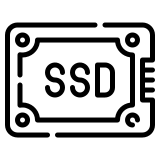
\includegraphics[width=0.8cm]{pictures/ssd}}

\colorlet{alicecolor}{green!90!black}
\colorlet{bobcolor}{red!90!black}
\colorlet{faustocolor}{yellow!90!black}
\colorlet{lightred}{red!50!white}
\colorlet{verylightgray}{gray!25!white}
      
\subtitle{Haute \'Ecole d'Informatique, Antananarivo, Madagascar, 4/11/2026}
\title{Hotmoka: The Ecological Blockchain}
\institute{Universit\`a di Verona, Italy}
\date{4/11/2026}

\setbeamercovered{invisible}

\def\codesize{\smaller}
\def\<#1>{\codeid{#1}}
\newcommand{\codeid}[1]{\ifmmode{\mbox{\codesize\ttfamily{#1}}}\else{\codesize\ttfamily #1}\fi}

\AtBeginSection[]{
  \begin{frame}
  \vfill
  \centering
  \begin{beamercolorbox}[sep=8pt,center,shadow=true,rounded=true]{title}
    \usebeamerfont{title}\insertsectionhead\par%
  \end{beamercolorbox}
  \vfill
  \end{frame}
}

\begin{document}

\begin{frame}
  \titlepage
\end{frame}

\begin{frame}{Blockchain?}

  A global database:
  \begin{itemize}
  \item transactions modify the state of the database
  \item transactions can be started by anybody, under payment
  \end{itemize}
  \bigskip
  The main properties of a blockchain:
  \begin{enumerate}
  \item immutability
  \item transparency
  \item censure-resistance
  \end{enumerate}

\end{frame}

\begin{frame}{Applications}
  Cryptocurrencies are just one of the applications of blockchain technology:
  \begin{itemize}
  \item decentralized money (Bitcoin, Ethereum, Cardano, Solana\ldots)
  \item decentralized smart contracts
  \item decentralized identities
  \item decentralized elections
  \item decentralized supply chains
  \item \ldots
  \end{itemize}
\end{frame}

\begin{frame}{The blockchain peer-to-peer network}

  \begin{center}
    \begin{tikzpicture}[scale=0.5,>=Stealth]
      \draw[thick] (-10,0) -- (0,3.5) -- (10,0) -- cycle;

      \draw (-10,0) node[above=0.2] {\computer} node[below=0.2,fill=faustocolor] {Fausto};
      \only<2>{\draw (-7.5,1.7) node[above] {\leftArrow};}
      \only<2>{\draw (-6,2.5) node[above] {{\tiny\signature\ Alice $\xRightarrow{100}$ Donald}};}
      \draw (-10.5,3.5) rectangle +(1,0.5) [fill=gray!30!white];
      \draw[->] (-10,4.5) -- +(0,-0.5);
      \draw (-10.5,4.5) rectangle +(1,0.5) [fill=pink!70!white];
      \draw[->] (-10,5.5) -- +(0,-0.5); 
      \draw (-10.5,5.5) rectangle +(1,0.5) [fill=blue!30!white];
      \only<3->{\draw[->] (-10,6.5) -- +(0,-0.5); 
        \draw (-10.5,6.5) rectangle +(1,0.5) [fill=brown!70!white];}

      \draw (10,0) node[above=0.2] {\computer} node[below=0.2,fill=bobcolor] {Bob};
      \draw (9.5,3.5) rectangle +(1,0.5) [fill=gray!30!white];
      \draw[->] (10,4.5) -- +(0,-0.5);
      \draw (9.5,4.5) rectangle +(1,0.5) [fill=pink!70!white];
      \draw[->] (10,5.5) -- +(0,-0.5); 
      \draw (9.5,5.5) rectangle +(1,0.5) [fill=blue!30!white];
      \only<3->{\draw[->] (10,6.5) -- +(0,-0.5); 
        \draw (9.5,6.5) rectangle +(1,0.5) [fill=brown!70!white];}

      \draw[->] (0,3.5) node[above=0.2] {\computer} node[below=0.2,fill=alicecolor] {Alice};
      \only<4>{\filldraw [fill=gray!10!white] (0,8.25) circle [radius=1,very thick];}
      \only<2>{\draw (2.5,3.7) node[above] {\leftArrow};}
      \only<2>{\draw (4,4.5) node[above] {{\tiny\signature\ Donald $\xRightarrow{2500}$ John}};}
      \draw (-0.5,7) rectangle +(1,0.5) [fill=gray!30!white];
      \draw[->] (0,8) -- +(0,-0.5);
      \draw (-0.5,8) rectangle +(1,0.5) [fill=pink!70!white];
      \draw[->] (0,9) -- +(0,-0.5);
      \draw (-0.5,9) rectangle +(1,0.5) [fill=blue!30!white];
      \visible<3->{\draw[->] (0,10) -- +(0,-0.5); 
        \draw (-0.5,10) rectangle +(1,0.5) [fill=brown!70!white];}

    \end{tikzpicture}
  \end{center}

  \begin{center}
    \only<1>{Each peer holds a private copy of the same blockchain data structure}
    \only<2>{Users can send signed transactions to any peer}
    \only<3>{Such transactions get eventually boxed into new blocks}
    \only<4>{Let us inspect a block of the blockchain}
  \end{center}

\end{frame}

\begin{frame}{Blocks}
  \begin{center}
    \begin{tikzpicture}[scale=0.9]
      \visible<2->{\draw [decorate,decoration={brace,amplitude=4pt},thick,xshift=0.3cm,yshift=0pt]
        (4.5,6.5) -- (4.5,4.5) node [midway,right,xshift=.2cm] {trunk};}
      \only<1-13,15->{\draw [fill=VioletRed, thick] (0,5.5) rectangle +(4.5,1);}
      \only<14>{\shadedraw [inner color=VioletRed,outer color=white, draw=black, thick] (0,5.5) rectangle +(4.5,1);}
      \draw (2.25,6) node{height};
      \draw [fill=VioletRed, thick] (0,4.5) rectangle +(4.5,1);
      \visible<2->{\draw (2.25,5) node{$\pi$ (creator's key)};}
      \only<1-12,14->{\draw [fill=Yellow, thick] (0,3.5) rectangle +(4.5,1);}
      \only<13>{\draw [inner color=Yellow,outer color=white, draw=black, thick] (0,3.5) rectangle +(4.5,1);}
      \only<3->{\draw (2.25,4) node{$\previousblockhash$};}
      \only<-3>{\phantom{\draw[->,thick] (0,4) -- (-1,4) node [midway,left,xshift=-.5cm] {$\previous$};}}
      \only<3->{\draw[->,thick] (0,4) -- (-1,4) node [midway,left,xshift=-.5cm] {$\previous$};}

      \draw [fill=Yellow, thick] (0,2.5) rectangle +(4.5,1);
      \visible<4->{\draw (2.25,3) node{nonce\,(arbitrary data)};}
      \only<1-14,17->{\draw [fill=Yellow, thick] (0,1.5) rectangle +(4.5,1);}
      \only<15,16>{\draw [inner color=Yellow,outer color=white, draw=black, thick] (0,1.5) rectangle +(4.5,1);}
      \visible<5->{\draw (2.25,2) node{$\tau$ (creation time)};}

      \only<1-6,8-16>{\draw [fill=SpringGreen, thick] (0,-1) rectangle +(4.5,2.5);}
      \only<7,17,18>{\draw [inner color=SpringGreen,outer color=white, draw=black, thick] (0,-1) rectangle +(4.5,2.5);}
      \visible<6-7>{\draw (2.25,0.3) node{transactions};}
      \visible<8->{\draw (2.25,1.1) node{\signature\ Alice $\xRightarrow{100}$ Donald};}
      \visible<9->{\draw (2.25,0.5) node{\signature\ Fausto $\xRightarrow{500}$ John};}
      \visible<10->{\draw (2.25,-0.1) node{\signature\ Donald $\xRightarrow{350}$ Alice};}
      \visible<11->{\draw (2.25,-0.7) node{\signature\ Donald $\xRightarrow{2500}$ John};}
    \end{tikzpicture}
  \end{center}

  \begin{center}
    \only<1-6>{\phantom{Rule 2: $\previous$ actually exists (no dangling pointers)}}
    \only<7-11>{Let us inspect the list of transactions}
    \only<12>{Valid blocks satisfy all \alert{consensus rules}:}
    \only<13>{\alert{Rule 1:} $\previous$ actually exists (no dangling pointers)}
    \only<14>{\alert{Rule 2:} The height increases: $\height=\previous.\height+1$}
    \only<15>{\alert{Rule 3:} The creation time increases: $\previous.\tau<\tau$}
    \only<16>{\alert{Rule 4:} The creation time is not in the future: $\tau\le\tau_\now$}
    \only<17>{\alert{Rule 5:} Each transaction is correctly signed by its sender}
    \only<18>{\alert{Rule 6:} Senders hold the money that they send}
  \end{center}

\end{frame}

\begin{frame}{Peers create (``mine'') new blocks}

  \begin{center}
    \begin{tikzpicture}[scale=0.5,>=Stealth]

      \draw[thick] (-10,0) -- (0,3.5) -- (10,0) -- cycle;

      \draw (-10,0) node[above=0.2] {\computer} node[below=0.2,fill=faustocolor] {Fausto};
      \draw (-10.5,3.5) rectangle +(1,0.5) [fill=gray!30!white];
      \draw[->] (-10,4.5) -- +(0,-0.5);
      \draw (-10.5,4.5) rectangle +(1,0.5) [fill=pink!70!white];
      \draw[->] (-10,5.5) -- +(0,-0.5); 
      \draw (-10.5,5.5) rectangle +(1,0.5) [fill=blue!30!white];
      \visible<2-3,5,7-8,10>{\draw[->] (-10,6.5) -- +(0,-0.5);}
      \visible<9>{\draw[->] (-10.5,6.5) -- +(0.5,-0.5);}
      \visible<9>{\draw[->] (-9.5,6.5) -- +(-0.5,-0.5);}
      \visible<2-3,8>{\draw (-10.5,6.5) rectangle +(1,0.5) [fill=faustocolor];}
      \visible<5,10>{\draw (-10.5,6.5) rectangle +(1,0.5) [fill=alicecolor];}
      \visible<7>{\draw (-10.5,6.5) rectangle +(1,0.5) [fill=bobcolor];}
      \visible<9>{\draw (-11.2,6.5) rectangle +(1,0.5) [fill=faustocolor];}
      \visible<9>{\draw (-9.8,6.5) rectangle +(1,0.5) [fill=alicecolor];}

      \draw (10,0) node[above=0.2] {\computer} node[below=0.2,fill=bobcolor] {Bob};
      \draw (9.5,3.5) rectangle +(1,0.5) [fill=gray!30!white];
      \draw[->] (10,4.5) -- +(0,-0.5);
      \draw (9.5,4.5) rectangle +(1,0.5) [fill=pink!70!white];
      \draw[->] (10,5.5) -- +(0,-0.5); 
      \draw (9.5,5.5) rectangle +(1,0.5) [fill=blue!30!white];
      \visible<3,5-7,10>{\draw[->] (10,6.5) -- +(0,-0.5);}
      \visible<9>{\draw[->] (9.5,6.5) -- +(0.5,-0.5);}
      \visible<9>{\draw[->] (10.5,6.5) -- +(-0.5,-0.5);}
      \visible<3>{\draw (9.5,6.5) rectangle +(1,0.5) [fill=faustocolor];}
      \visible<5,10>{\draw (9.5,6.5) rectangle +(1,0.5) [fill=alicecolor];}
      \visible<6-7>{\draw (9.5,6.5) rectangle +(1,0.5) [fill=bobcolor];}
      \visible<9>{\draw (8.8,6.5) rectangle +(1,0.5) [fill=faustocolor];}
      \visible<9>{\draw (10.2,6.5) rectangle +(1,0.5) [fill=alicecolor];}

      \draw (0,3.5) node[above=0.2] {\computer} node[below=0.2,fill=alicecolor] {Alice};
      \draw (-0.5,7) rectangle +(1,0.5) [fill=gray!30!white];
      \draw[->] (0,8) -- +(0,-0.5);
      \draw (-0.5,8) rectangle +(1,0.5) [fill=pink!70!white];
      \draw[->] (0,9) -- +(0,-0.5);
      \draw (-0.5,9) rectangle +(1,0.5) [fill=blue!30!white];
      \visible<3-5,7-8,10>{\draw[->] (0,10) -- +(0,-0.5);}
      \visible<9>{\draw[->] (-0.5,10) -- +(0.5,-0.5);}
      \visible<9>{\draw[->] (0.5,10) -- +(-0.5,-0.5);}
      \visible<3>{\draw (-0.5,10) rectangle +(1,0.5) [fill=faustocolor];}
      \visible<4-5,8,10>{\draw (-0.5,10) rectangle +(1,0.5) [fill=alicecolor];}
      \visible<7>{\draw (-0.5,10) rectangle +(1,0.5) [fill=bobcolor];}
      \visible<9>{\draw (-1.2,10) rectangle +(1,0.5) [fill=faustocolor];}
      \visible<9>{\draw (0.2,10) rectangle +(1,0.5) [fill=alicecolor];}

    \end{tikzpicture}
  \end{center}

  \begin{overprint}
    \onslide<2-3>
    \centering Fausto creates a new block\ldots
    \onslide<4-5>
    \centering \ldots or Alice creates a new block
    \onslide<6-7>
    \centering \ldots or Bob creates a new block
    \onslide<8-9>
    \centering \ldots or Fausto and Alice create a new block!
    \onslide<10>
    \centering Peers select the \emph{best} block
  \end{overprint}

\end{frame}

\begin{frame}{Blockchain mining as a competitive puzzle}

  Mining of a \textbf{next} block on top of a \textbf{block}:
  \quad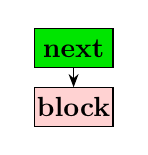
\begin{tikzpicture}[scale=0.5,>=Stealth]
    \draw (0,1.5) rectangle +(2,1) [fill=alicecolor];
    \draw[->] (1,1.5) -- +(0,-0.5);
    \draw (0,0) rectangle +(2,1) [fill=pink!70!white];
    \draw (1,0) node[above] {\textbf{block}};
    \draw (1,1.5) node[above] {\textbf{next}};
  \end{tikzpicture}

  \begin{description}
  \item[{\color{red}challenge:}] \only<2->{derive (deterministically) a challenge from the \textbf{block}}
  \item[{\color{red}answer:}] \only<3->{send all peers a \textbf{next} that satisfies the challenge}
  \item[{\color{red}competition:}] \only<4->{in case of more \textbf{next}, select a \emph{best} one}
  \end{description}

  \bigskip

  \visible<5->{Bitcoin's Proof of Work (PoW): best means \emph{with some arbitrary data (nonce) that minimizes the hash of the block}}

\end{frame}

\begin{frame}\frametitle{Annualized Bitcoin's total footprint}

  \begin{center}
    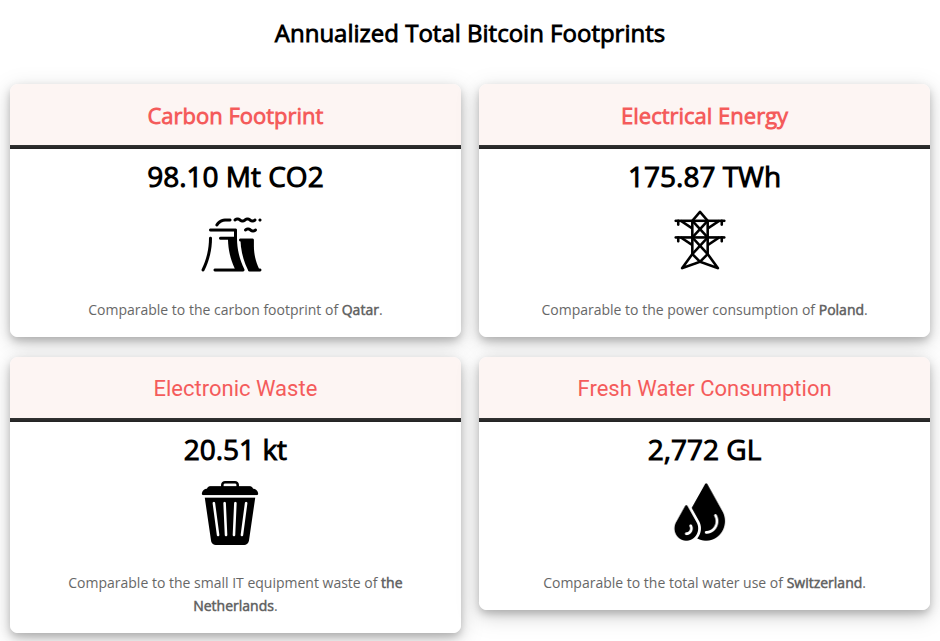
\includegraphics[width=0.85\textwidth,clip=false]{pictures/footprint-annual}
  \end{center}

  \begin{center}
    {\tiny (source: \url{https://digiconomist.net/bitcoin-energy-consumption})}
  \end{center}

\end{frame}

\begin{frame}{Blockchain mining as a competitive puzzle}

  Mining of a \textbf{next} block on top of a \textbf{block}:
  \quad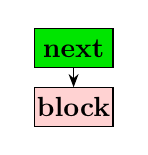
\begin{tikzpicture}[scale=0.5,>=Stealth]
    \draw (0,1.5) rectangle +(2,1) [fill=alicecolor];
    \draw[->] (1,1.5) -- +(0,-0.5);
    \draw (0,0) rectangle +(2,1) [fill=pink!70!white];
    \draw (1,0) node[above] {\textbf{block}};
    \draw (1,1.5) node[above] {\textbf{next}};
  \end{tikzpicture}

  \begin{description}
  \item[{\color{red}challenge:}] derive (deterministically) a challenge from the \textbf{block}
  \item[{\color{red}answer:}] send all peers a \textbf{next} that satisfies the challenge
  \item[{\color{red}competition:}] in case of more \textbf{next}, select a \emph{best} one
  \end{description}

  \bigskip

  Bitcoin's Proof of Work (PoW): best means \emph{with some arbitrary data (nonce) that minimizes the hash of the block}

  \pause
  \bigskip

  Mokamint's Proof of Space (PoSp): best means \emph{with some data (nonce) from a precomputed set (plot) that minimizes a delay function}

\end{frame}

\begin{frame}\frametitle{Proof of Work vs.\ Proof of Space}

  \begin{greenbox}{Mining for Proof of Work}
    \begin{itemize}
    \item fully decentralized, high computational cost, minimal disk usage
    \item efficient code already exists (Bitcoin)
    \item remote mining is hard (large bandwidth)
    \item it needs significant investment, energy, good networking
    \item extremely unlikely in a poor country
    \end{itemize}
  \end{greenbox}

  \pause
  \medskip

  \begin{greenbox}{Mining for Proof of Space}
    \begin{itemize}
    \item fully decentralized, minimal computational cost, high disk usage
    \item only vertical undocumented code exist
    \item remote mining is easy (minimal bandwidth)
    \item it needs no investment, almost no energy, minimal bandwidth
    \item possible also in poor countries
    \end{itemize}
  \end{greenbox}
\end{frame}

\begin{frame}{Mokamint (Fausto Spoto, 2023--2025)}

  \begin{center}
    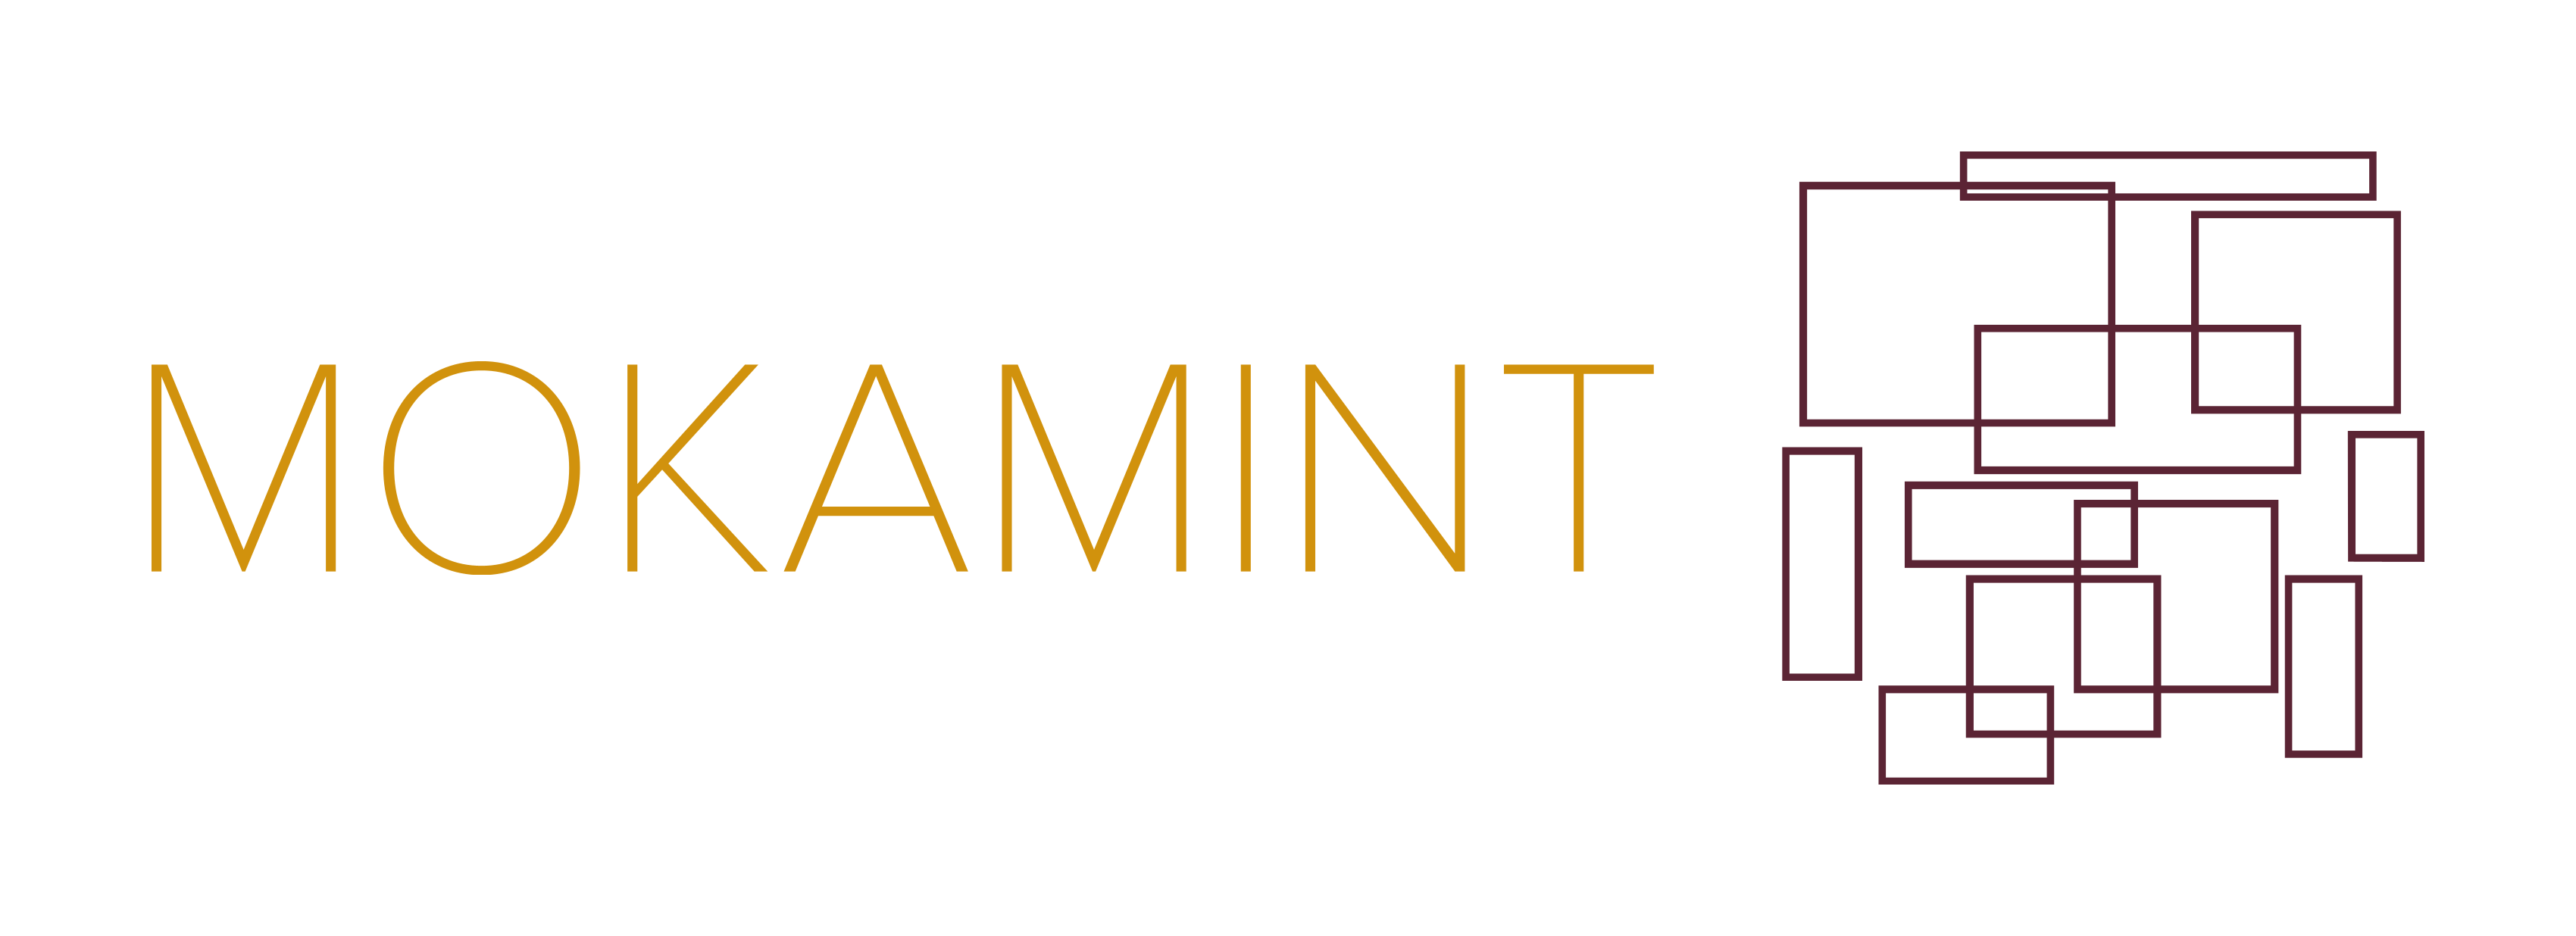
\includegraphics[width=0.4\textwidth]{pictures/mokamint_logo}\\
    \url{https://github.com/Mokamint-chain/mokamint}
  \end{center}

  \begin{center}
    A new open-source (Apache 2.0) blockchain based on proof of space, \alert{generic}
    wrt.\ the supported \alert{application}
  \end{center}

  \medskip

  \begin{center}
    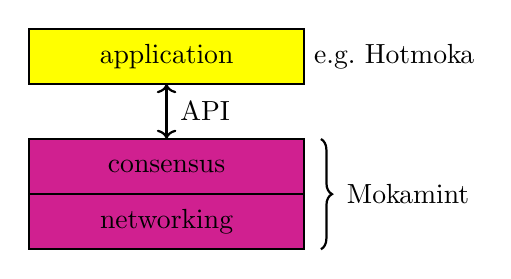
\begin{tikzpicture}[scale=0.7]
      \draw [fill=VioletRed, thick] (0,0) rectangle +(5,1);
      \draw (2.5,0.5) node{networking};
      \draw [fill=VioletRed, thick] (0,1) rectangle +(5,1);
      \draw (2.5,1.5) node{consensus};
      \draw[<->, thick] (2.5,2) -- (2.5,3);
      \draw (3.2,2.5) node{API};
      \draw [fill=Yellow, thick] (0,3) rectangle +(5,1);
      \draw (2.5,3.5) node{application};
      \draw (5,3.5) node [right] {e.g.\ Hotmoka};
      \draw [decorate,decoration={brace,amplitude=4pt},thick,xshift=0.3cm,yshift=0pt]
      (5,2) -- (5,0) node [midway,right,xshift=.2cm] {Mokamint};
    \end{tikzpicture}
  \end{center}

\end{frame}

\begin{frame}{Hotmoka (Fausto Spoto et al., 2019--2026)}

  \begin{center}
    
\includegraphics[width=0.4\textwidth]{pictures/hotmoka_logo}\\
    \url{https://github.com/Hotmoka/hotmoka}
  \end{center}

  \begin{center}
    An open-source (Apache 2.0) software layer for the execution of \alert{smart contracts} written in a subset of Java
  \end{center}

  \medskip

  \begin{center}
    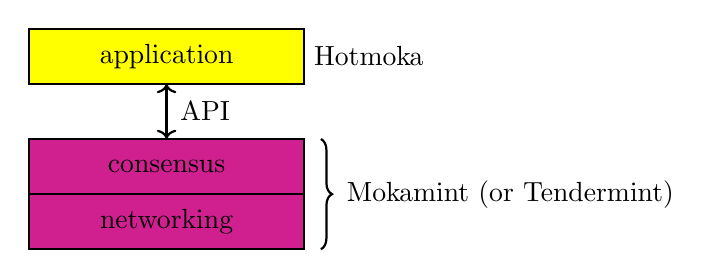
\begin{tikzpicture}[scale=0.7]
      \draw [fill=VioletRed, thick] (0,0) rectangle +(5,1);
      \draw (2.5,0.5) node{networking};
      \draw [fill=VioletRed, thick] (0,1) rectangle +(5,1);
      \draw (2.5,1.5) node{consensus};
      \draw[<->, thick] (2.5,2) -- (2.5,3);
      \draw (3.2,2.5) node{API};
      \draw [fill=Yellow, thick] (0,3) rectangle +(5,1);
      \draw (2.5,3.5) node{application};
      \draw (5,3.5) node [right] {Hotmoka};
      \draw [decorate,decoration={brace,amplitude=4pt},thick,xshift=0.3cm,yshift=0pt]
      (5,2) -- (5,0) node [midway,right,xshift=.2cm] {Mokamint (or Tendermint)};
    \end{tikzpicture}
  \end{center}

\end{frame}

\begin{frame}[fragile]{The Mokamint+Hotmoka blockchain}

  Currently composed of six peers
  \medskip

  \begin{greenbox}{\texttt{mokamint-node peers ls --uri ws://lipari.hotmoka.io:8030}}
\begin{verbatim}
ws://157.90.103.251:8032    1000  connected
 ws://84.32.9.124:8030      1000  connected
 ws://84.32.9.193:8030      1000  connected
 ws://88.216.93.12:8030     1000  connected
 ws://93.115.28.68:8030     1000  connected
\end{verbatim}
  \end{greenbox}

\end{frame}

\medskip

\begin{frame}[fragile]{The Mokamint+Hotmoka blockchain}

  \begin{greenbox}{\texttt{mokamint-node chain ls 4 from 0 --uri ws://lipari.hotmoka.io:8030}}
\begin{verbatim}
3: adb...1  2026-03-21 15:00:27  HdP...c  CFK...F
2: bff...a  2026-03-21 15:00:27  HdP...c  CFK...F
1: 314...2  2026-03-21 15:00:27  HdP...c  CFK...F
0: ebc...d  2026-03-21 15:00:27  HdP...c    ---                     
\end{verbatim}
  \end{greenbox}

  \pause
  \bigskip

  \begin{greenbox}{\texttt{mokamint-node chain ls 4 --uri ws://lipari.hotmoka.io:8030}}
\begin{verbatim}
968584: c16...5  2026-11-02 15:47:59  31g...o  CfY...7
968583: a85...d  2026-11-02 15:47:43  3Wq...T  5Z5...D
968582: 2fa...3  2026-11-02 15:47:35  tQ6...r  9CF...r
968581: 428...a  2026-11-02 15:46:46  31g...o  CfY...7
\end{verbatim}
  \end{greenbox}
\end{frame}

\begin{frame}\frametitle{Miners as mobile applications}

  \begin{center}
    \begin{tikzpicture}[scale=1]
      \draw [fill=verylightviolet,thick] (-0.5,0) rectangle +(4,1.5);
      \draw (1.5,1.1) node {blockchain peer};
      \draw (1.5,0.5) node {\textbf{Mokamint}};
      \draw (1.5,2.2) node[scale=0.7] {\computer};
      \draw (-1.5,0.8) node[scale=0.7] {\db};

      \draw [fill=verylightred,thick] (7,0.15) rectangle +(3,1.2);
      \draw (8.5,1) node {miner(s)};
      \draw (8.5,0.5) node {\textbf{Mokaminter}};
      \draw (8.5,2.1) node[scale=0.7] {\phone};

      \draw[->, thick] (3.5,1.0) -- (7,1.0);
      \draw (5.25,1.25) node {{\small challenges}};

      \draw[<-, thick] (3.5,0.5) -- (7,0.5);
      \draw (5.25,0.25) node {{\small answers (nonces)}};

    \end{tikzpicture}
  \end{center}

  \begin{center}
    \alert{Can we do it for PoSp (Mokamint, at least) ?}
  \end{center}

  \pause

  \begin{itemize}
  \item yes, since PoSp uses almost no CPU during the mining phase
    \begin{itemize}
    \item this preserves the battery of the device
    \end{itemize}
  \item yes, since challenges are a around $64$ bytes long and nonces can be compacted into
    \emph{deadlines} of around $200$ bytes
    \begin{itemize}
    \item this limits the bandwith needed during mining
    \end{itemize}
  \item yes, average mobile devices have around $256~GB$ of SSD, compared to
    an average of $1000~GB$ of SSD of desktop computers
    \begin{itemize}
    \item mining can still be competitive on a mobile device
    \end{itemize}
  \end{itemize}
  
\end{frame}

\begin{frame}\frametitle{5G coverage in Brazil}
  \begin{center}
    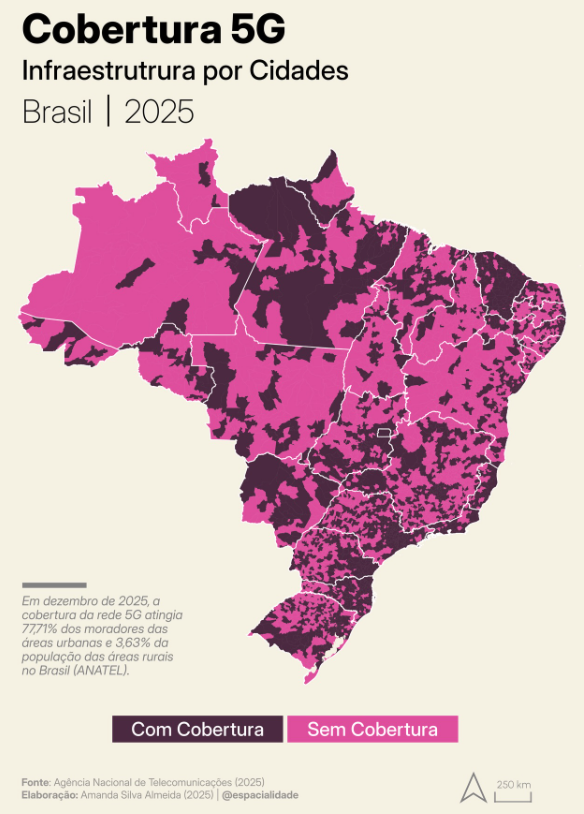
\includegraphics[width=5.6cm]{pictures/5g}
  \end{center}
\end{frame}

\begin{frame}\frametitle{Mokaminter: mobile mining on Android}

  \begin{center}
    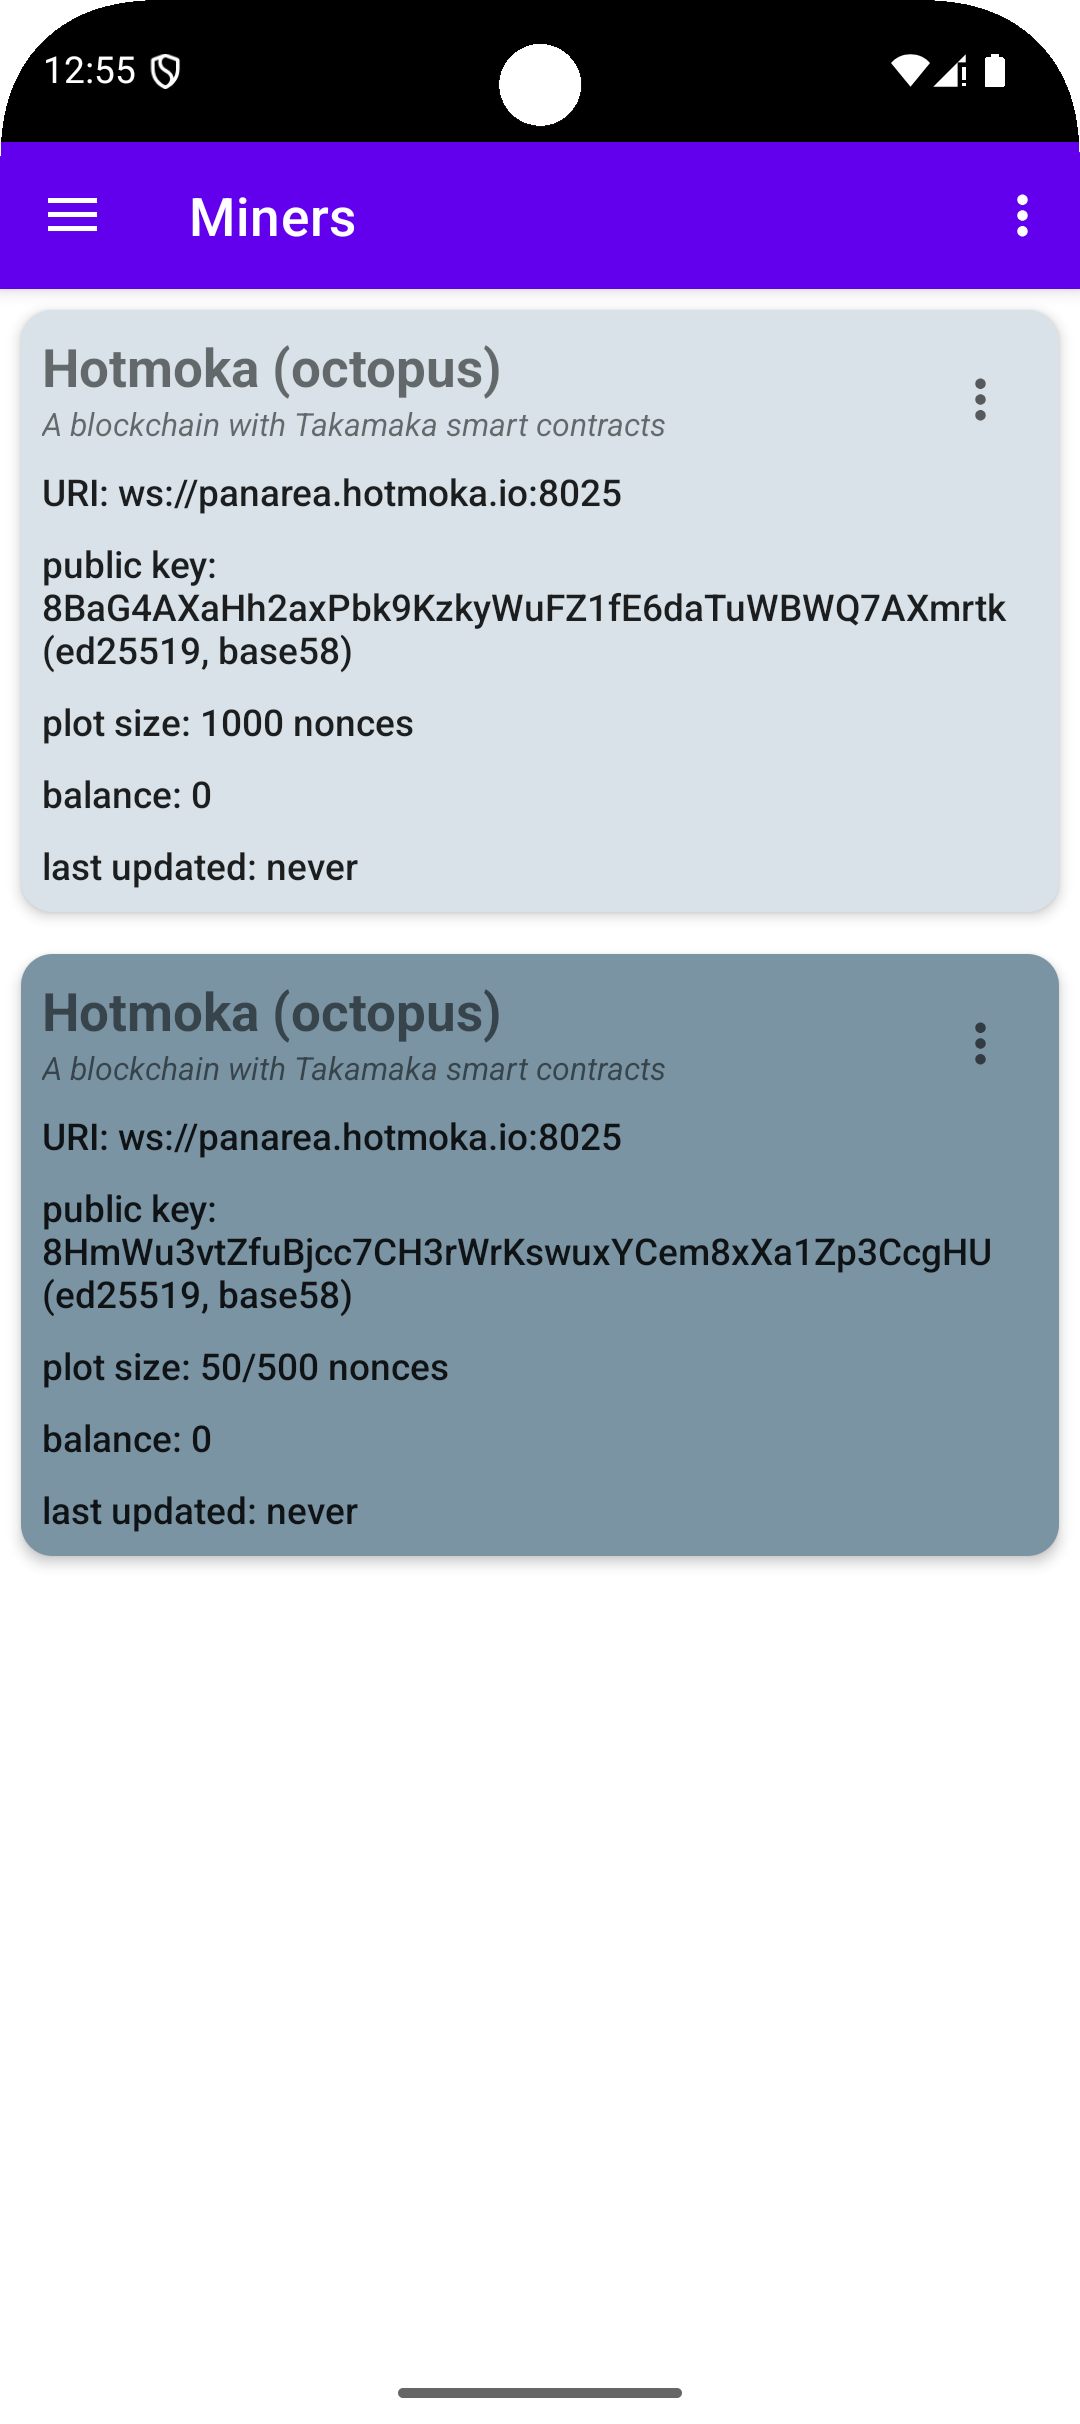
\includegraphics[width=5.6cm]{pictures/mokaminter}
  \end{center}

\end{frame}

\begin{frame}\frametitle{Mokaminter: crypto (mokas) earned after 24h of mining}

  \begin{center}
    \hspace*{-1.5ex}\begin{tabular}{r|r|r|c|c|c}
      {\small crypto} & disk & {\small CPU} & model & kind & region\\\hline\hline
      276 & 0.17MB & 5\% & {\small Motorola edge 40 neo} & phone & Italy\\\hline
      310 & 3MB & 2\% & {\small Poco F4} & phone & Italy\\\hline
      138 & 0MB & 0\% & {\small Samsung Galaxy S24} & phone & Brazil \\\hline
       68 & 0.49MB & 0\% & {\small Samsung Galaxy S25 ultra} & phone & Italy\\\hline
      103 & 6.1MB & 0\% & {\small Samsung Galaxy Tab S11} & tablet & Italy\\\hline
      310 & 0MB & 6\% & {\small Xiaomi 11 Lite 5G NE} & phone & Italy\\\hline
       68 & 4.77MB & 5\% & {\small Samsung Galaxy Tab A9+} & tablet & Spain\\\hline
      103 & 0MB & 6\% & {\small Redmi Note 8T} & phone & Italy\\\hline
      413 & 3.18MB & 4\% & {\small Lenovo Tab M11 TB330XU} & tablet & Italy\\\hline
      103 & 1.06MB & 1\% & {\small Samsung Galaxy Tab S6 Lite} & tablet & Italy\\\hline
       68 & 0.13MB & 0\% & {\small Motorola edge 40 neo} & phone & La R\'eunion\\\hline
      170 & 2.20MB & 6\% & {\small Motorola edge 40 neo} & phone & Madagascar
    \end{tabular}
  \end{center}

\end{frame}

\begin{frame}\frametitle{Take part in the evaluation of Mokaminter}

  \begin{center}
    
\includegraphics[width=0.3\textwidth,clip=false]{pictures/I_want_you}
  \end{center}

  Install Mokaminter from Google Play on your Android device and use it
  for 24 hours for mining for Hotmoka

  \medskip

  Send me statistics at the end

  \medskip

  Instructions at \url{https://www.hotmoka.io/Mokaminter_EN.pdf}

\end{frame}

\begin{frame}\frametitle{Your help with Hotmoka is welcome!}

  \begin{itemize}
  \item Do you want to use your Android device as a miner and earn crypto?
    Install Mokaminter:
    \url{https://play.google.com/store/apps/details?id=io.mokamint.android.mokaminter}
  \item Do you want to use your computer as a miner and earn crypto? Install a desktop miner: \url{https://hub.docker.com/r/mokamint/mokamint}
  \item Do you want your computer to become a peer of the network?
    Install Mokamint and Hotmoka:
    \url{https://hub.docker.com/r/hotmoka/mokamint-node}
  \end{itemize}

  \begin{center}
    Documentation and tutorial:\\
    \url{https://hotmoka.io}\\
    \url{https://www.hotmoka.io/tutorial}
  \end{center}
\end{frame}

\end{document}
